 % !TeX program = xelatex
\documentclass[12pt]{article}
\usepackage[margin=2.5cm]{geometry}
\usepackage{array}
\usepackage{longtable}
\usepackage{graphicx}
\usepackage{hyperref}
\usepackage{titlesec}
\usepackage{enumitem}
\usepackage{booktabs}
\usepackage{fontspec}
\setmainfont{Noto Sans}

% Compact formatting tweaks to keep Section 2 on page 1
\usepackage{microtype}
\usepackage{ragged2e}
\setlength{\parindent}{0pt}
\setlength{\parskip}{0.35em}
\usepackage{titlesec}
\titlespacing*{\section}{0pt}{0.75em}{0.5em}
\titlespacing*{\subsection}{0pt}{0.6em}{0.4em}
\setlength{\LTpre}{0pt}
\setlength{\LTpost}{0pt}
\setlength{\abovecaptionskip}{4pt}
\setlength{\belowcaptionskip}{6pt}

\title{Week 2 Progress Report — OIP Sentinel (Firestore + Aerospike)}
\author{}
\date{\today}

\begin{document}
% Header styled like the provided sample
\begin{center}
\Large\textbf{Progress Report for Project Consultation}
\end{center}

% Centered rule under the main heading (slightly shorter than text width)
\noindent\makebox[\textwidth]{\rule{0.92\textwidth}{0.8pt}}
\vspace{0.6em}

\vspace{0.5em}
\begin{flushleft}
\textbf{Title of the Project:} OIP Sentinel — Distributed Database (Firestore + Aerospike)\\
\textbf{Group Name:} Sharpness\\[0.6em]
\textbf{Members:}\\
Faustino Sotomayor (Leader)\\
Erika Bicoy (Member)\\
Mark Angelo Dontar (Member)\\
Sanny Fhel Paalisbo (Member)\\
Jomari Sunogan (Member)\\[0.6em]
\noindent\rule{\textwidth}{0.4pt}\\[0.4em]
\textbf{Date:} \today\ (e.g., \today)
\end{flushleft}
\vspace{0.5em}

\section{Executive Summary and Project Status}
This week we solidified authentication with RBAC, 2FA (email OTP), and trusted devices; expanded the backend database manager bridging Firestore and Aerospike; and validated audit logging for admin and cashier streams. Screenshots below evidence working flows. Next, we will add pagination for Aerospike scans and structured logging.

\section{System Overview}

\subsection{Features Implemented (or Planned)}
% Slightly smaller table font and tighter columns
\begingroup\small\setlength{\tabcolsep}{6pt}
\begin{longtable}{p{0.35\linewidth} p{0.6\linewidth}}
\caption{Table 1: Project Feature Status Summary}\\
\toprule
\textbf{Feature Name} & \textbf{Status and Progress} \\
\midrule
User Authentication (Sign Up/Login) & Completed. Email/password and Google Sign-In; role/status enforcement. \\
RBAC (Admin/Cashier) & Completed. Firestore roles with UI gating and cached role. \\
2FA (OTP + Trusted Devices) & Completed. Email OTP; device trust window under user subcollection. \\
Audit Logging & Completed. Admin and cashier logs to Firestore with device metadata. \\
Backend DB Manager (REST) & Completed. List/insert/read across Firestore and Aerospike; CORS enabled. \\
Aerospike Integration & Completed. Namespace \texttt{oipms}; key insert; normalized scan read. \\
Password Reset OTP & Client-ready; server endpoint planned. \\
ML Object Detection & Planned. Not implemented this week. \\
\bottomrule
\end{longtable}
\endgroup

\subsection{Database Integration}
\textbf{Technology:} Firebase Firestore (RBAC, OTP, audit), Aerospike (business data).\\
\textbf{Schema:} Firestore collections: \texttt{users}, \texttt{audit\_logs\_admin}, \texttt{audit\_logs\_cashier}, \texttt{\_loginOtps}, \texttt{tables}; Aerospike: namespace \texttt{oipms}, sets discovered dynamically.\\
\textbf{Integration Status:} Frontend CRUD/auth working; backend OTP and DB manager operational.\\
\textbf{Challenges:} Firestore indexes for identifier lookups; SendGrid/Twilio config; Aerospike pagination.

\section{Work Completed and Remaining Tasks}
\subsection{Completed Milestones}
\begin{itemize}[leftmargin=*]
  \item Auth with RBAC, OTP, and trusted-device refresh.
  \item Firestore audit logging (admin/cashier) with device details.
  \item Express backend: OTP endpoints and DB manager (FS/Aerospike).
  \item Aerospike inserts and normalized scan reads.
\end{itemize}
\subsection{Outstanding Tasks and Next Steps}
\begin{itemize}[leftmargin=*]
  \item Add pagination/filters to Aerospike reads; document scan costs.
  \item Add structured request logging and correlation IDs on backend.
  \item Document security rules and indexes; parameterize backend URL.
  \item Implement password-reset OTP server endpoint.
\end{itemize}

\section{Screenshot of the UI/UX}
\noindent\textbf{Note:} Images referenced from \texttt{docs/progress/images/}.

% --- Figure 1: Admin Dashboard ---
\begin{figure}[htbp]
  \centering
  \fbox{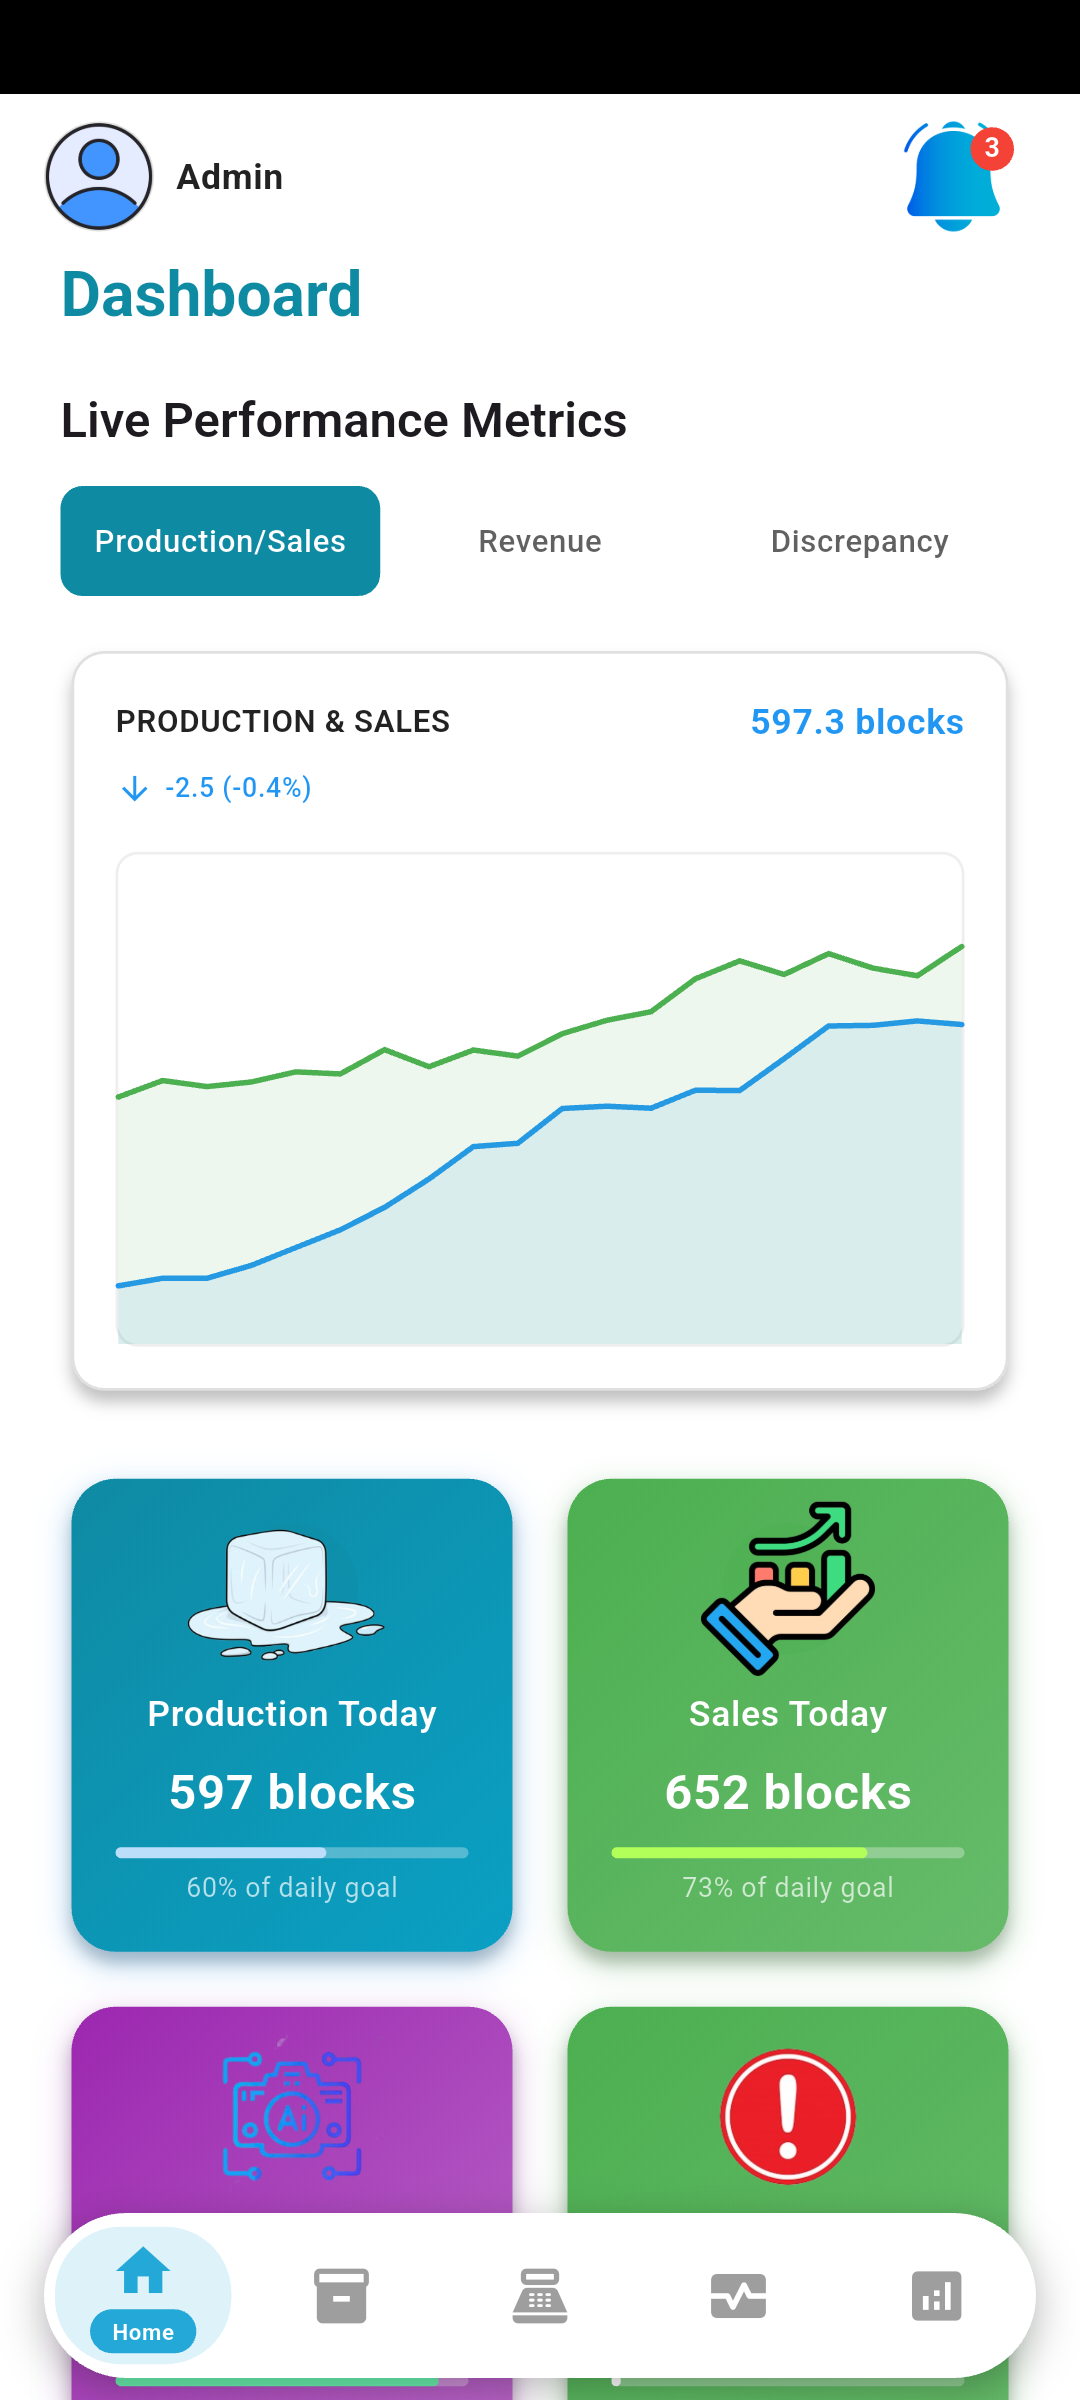
\includegraphics[width=\linewidth]{images/admin.png}}
  \caption{Primary Dashboard View (Admin): Role-based navigation, metrics, and administrative actions.}
  \label{fig:dashboard-admin}
\end{figure}

% --- Figure 2: Cashier Dashboard ---
\begin{figure}[htbp]
  \centering
  \fbox{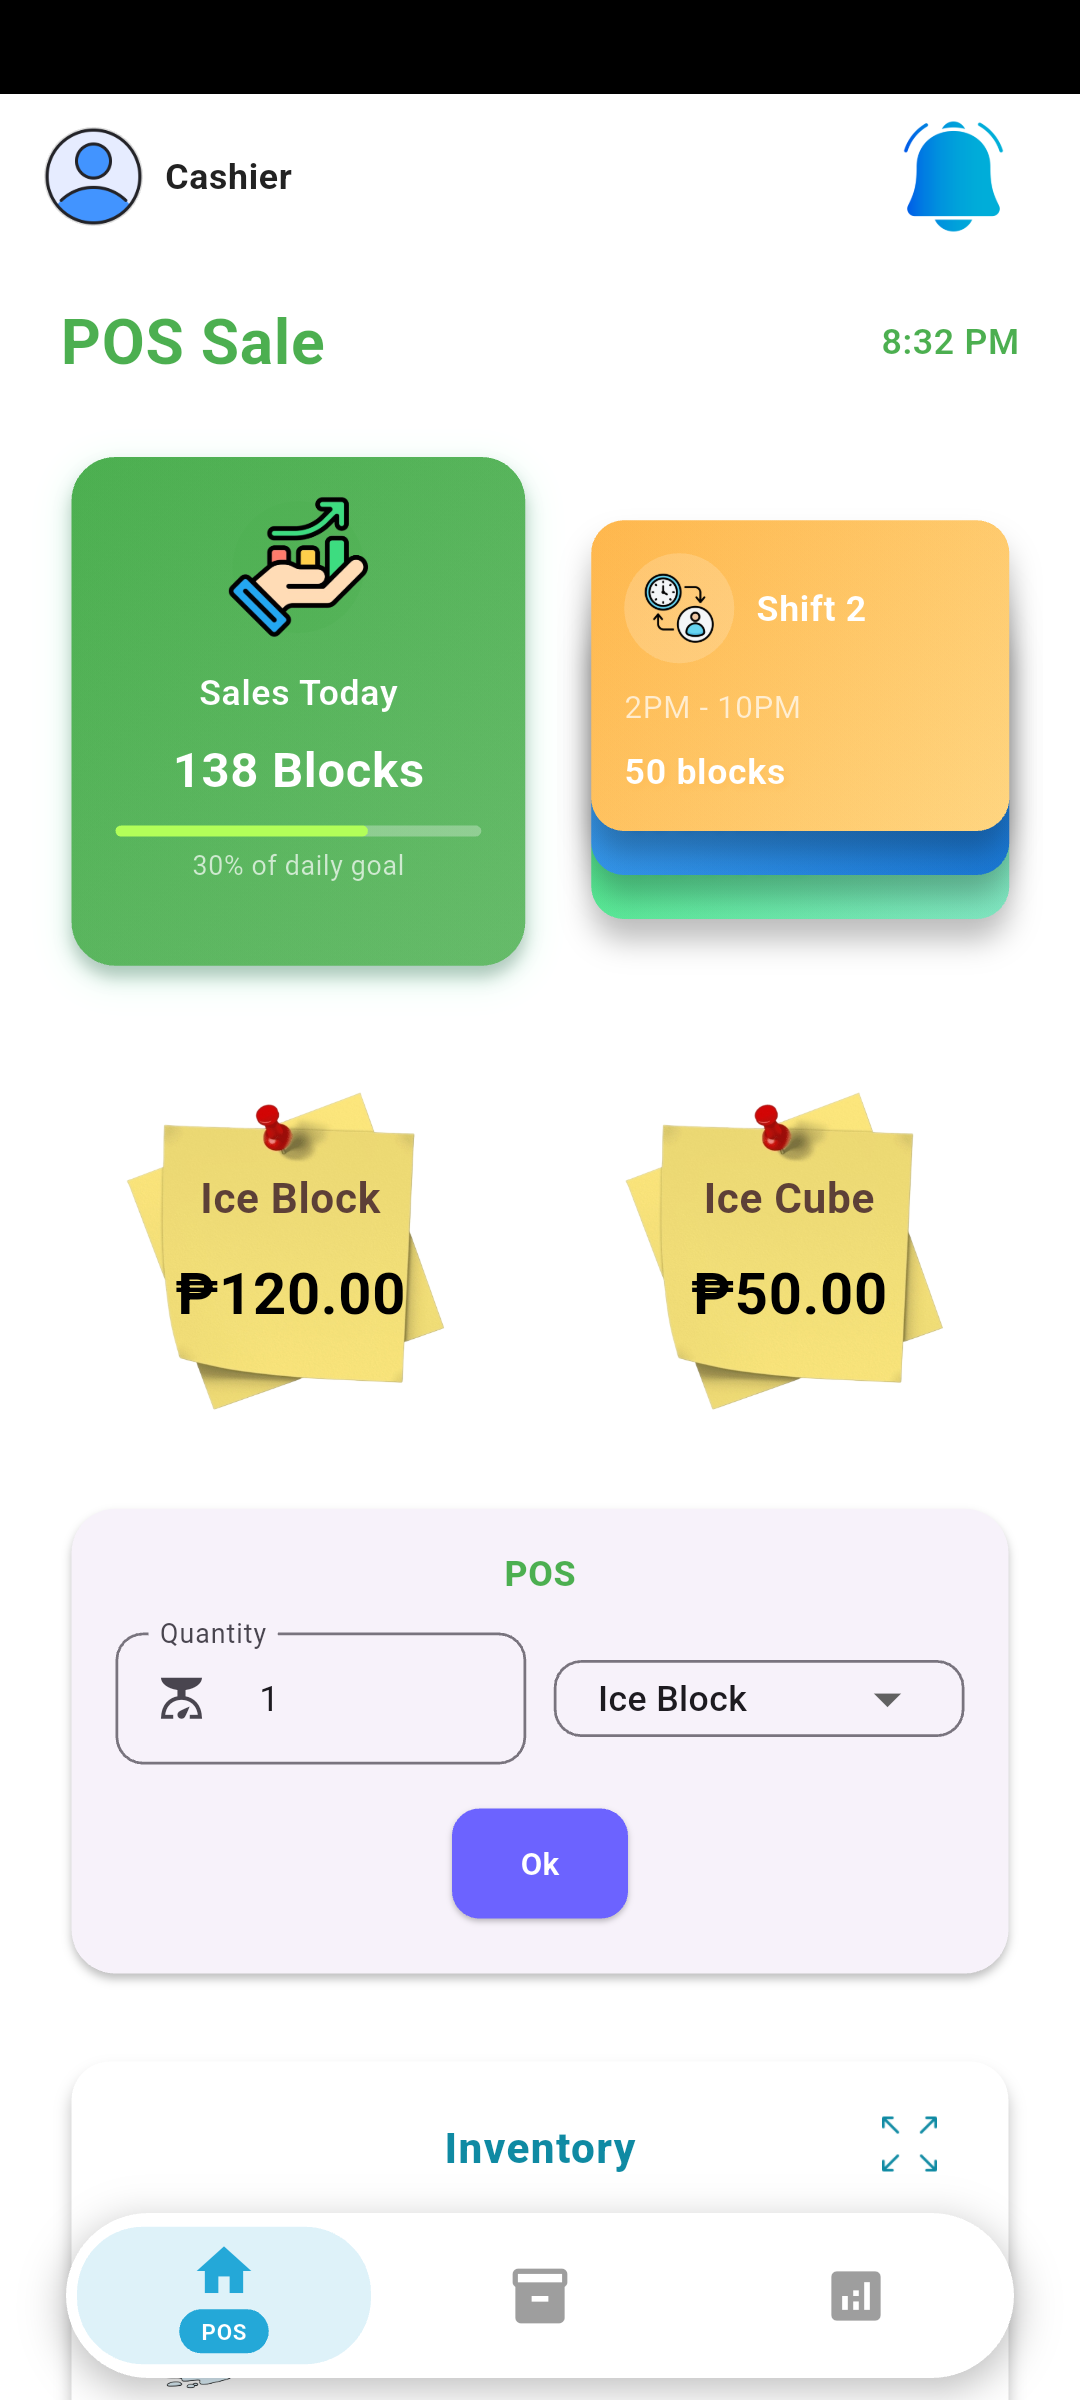
\includegraphics[width=\linewidth]{images/cashier.png}}
  \caption{Primary Dashboard View (Cashier): Cashier-focused layout and actions.}
  \label{fig:dashboard-cashier}
\end{figure}

% --- Figure 3: OTP (2FA) ---
\begin{figure}[htbp]
  \centering
  \fbox{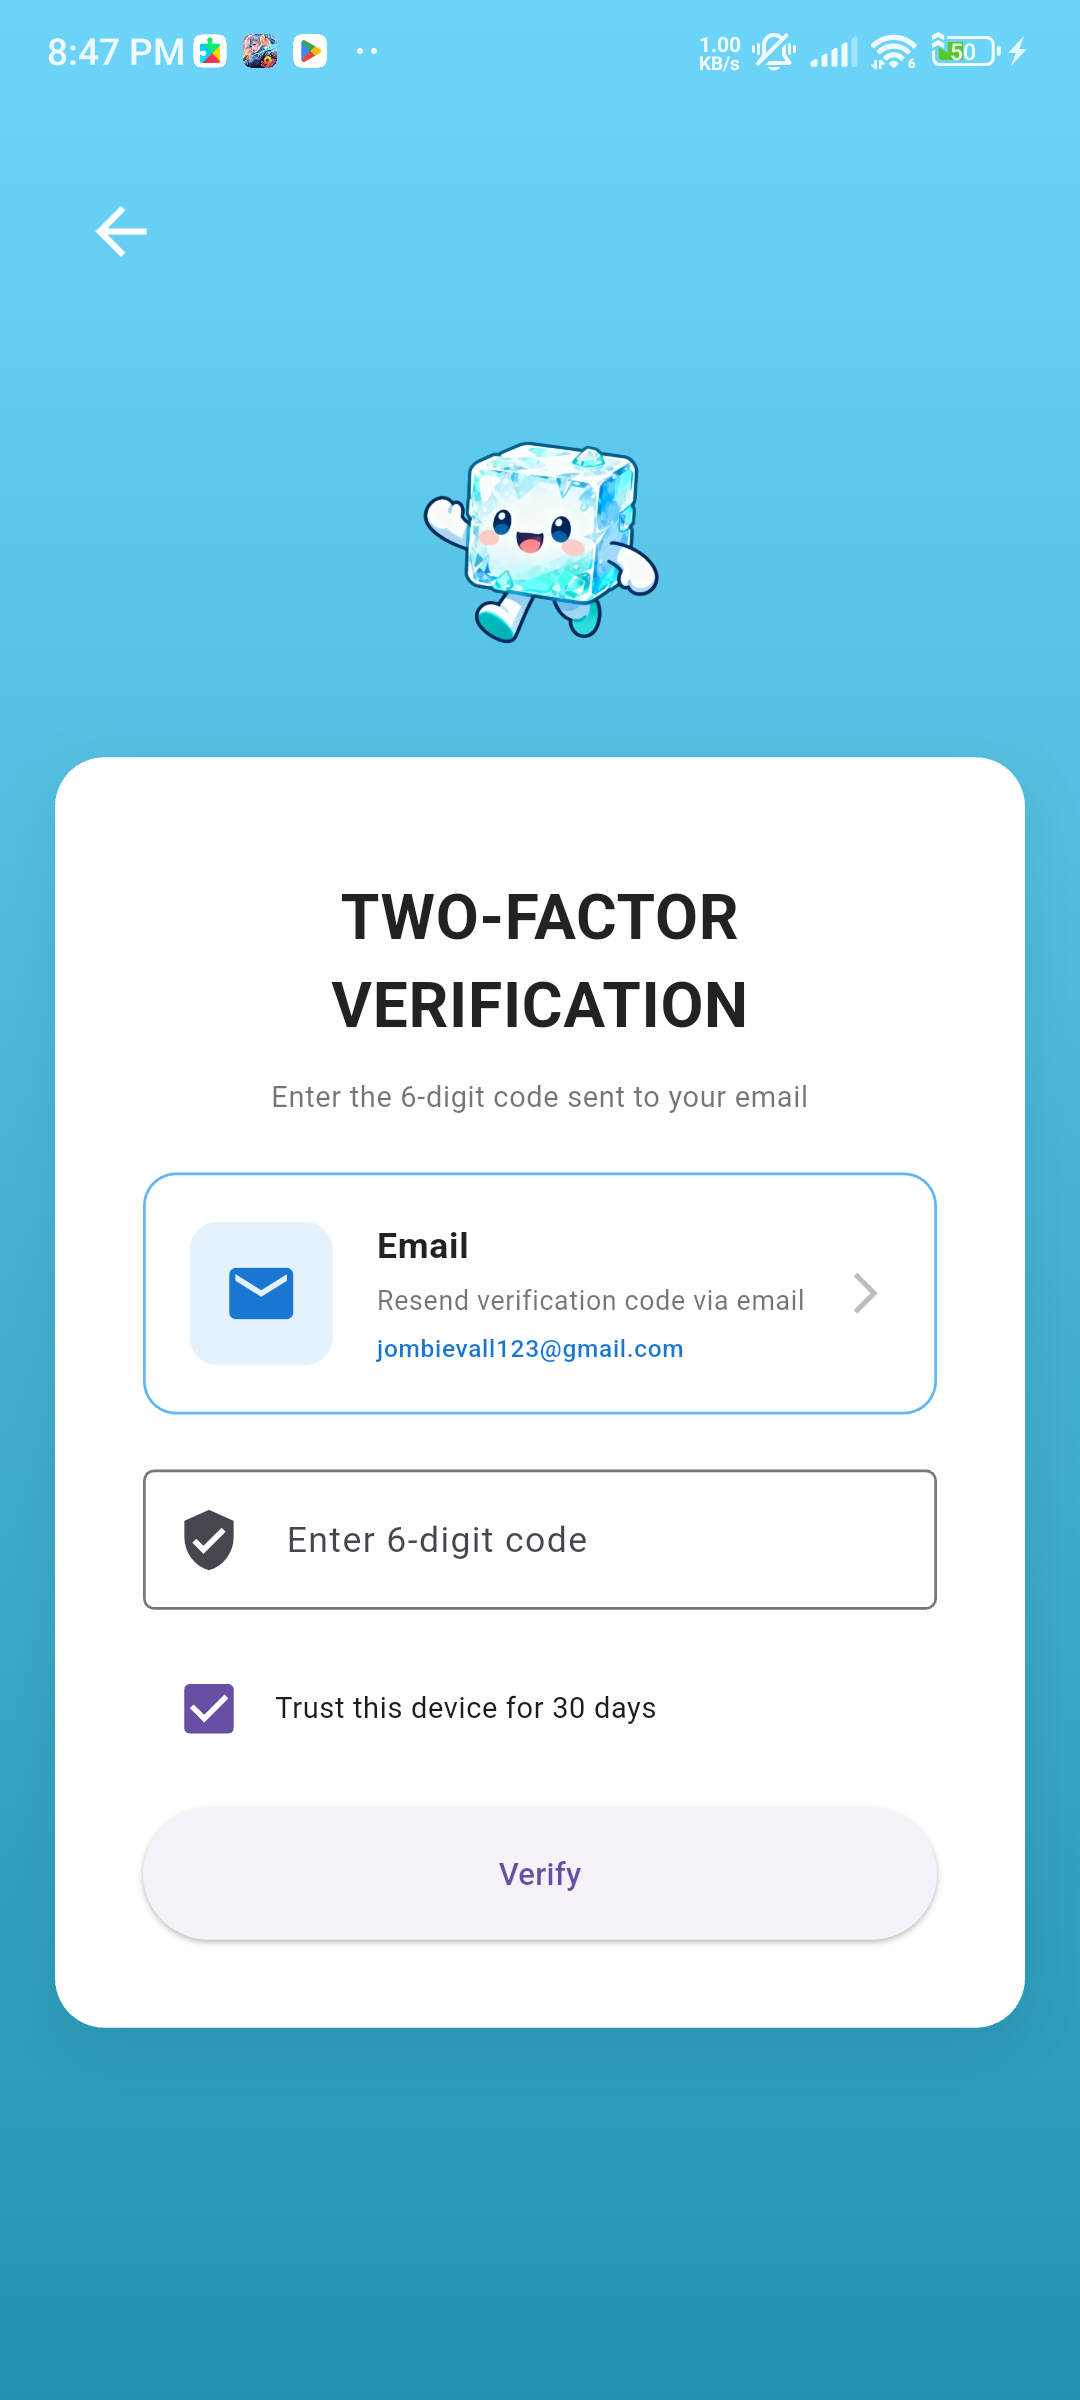
\includegraphics[width=\linewidth]{images/otp.png}}
  \caption{Data Input/Form View: Step-up email OTP verification with clear feedback.}
  \label{fig:otp}
\end{figure}

% --- Figure 4: DB Manager ---
\begin{figure}[htbp]
  \centering
  \fbox{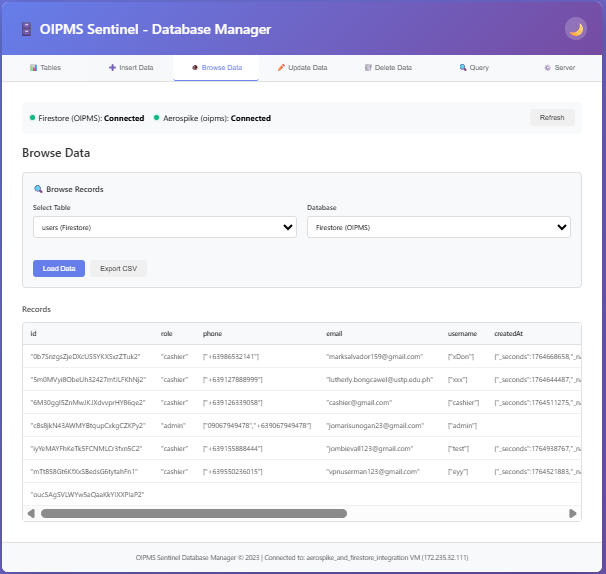
\includegraphics[width=\linewidth]{images/manager.png}}
  \caption{Database Manager: Listing tables and performing CRUD across Firestore and Aerospike.}
  \label{fig:db-manager}
\end{figure}

% --- Figure 5: Audit Trail (Admin) ---
\begin{figure}[htbp]
  \centering
  \fbox{
\includegraphics[width=\linewidth]{\detokenize{images/audit trail admin.png}}}
  \caption{Audit Trail (Admin): Normalized events including device and route metadata.}
  \label{fig:audit-admin}
\end{figure}

% --- Figure 6: Audit Trail (Cashier) ---
\begin{figure}[htbp]
  \centering
  \fbox{
\includegraphics[width=\linewidth]{\detokenize{images/audit trail cashier.png}}}
  \caption{Audit Trail (Cashier): Cashier-context events captured separately.}
  \label{fig:audit-cashier}
\end{figure}

\subsection{Screenshot 1: Primary Dashboard View}
See Figures~\ref{fig:dashboard-admin} and~\ref{fig:dashboard-cashier}.

\subsection{Screenshot 2: Data Input/Form View}
See Figure~\ref{fig:otp}.

\section{Challenges and Mitigation}
\begin{itemize}[leftmargin=*]
  \item CORS: Resolved via global middleware and OPTIONS handling.
  \item OTP delivery: Configured SendGrid/Twilio; non-enumerating responses.
  \item Aerospike namespace/listing: Limited to \texttt{oipms}; validated info parsing.
  \item RBAC consistency: Cashier approval enforced; safe role caching.
\end{itemize}

\section{Conclusion and Next Reporting Period}
End-to-end flows (auth, 2FA, audit, DB manager) are working. Next week focuses on pagination, structured logging, and security documentation.

\end{document}
